\section{Introduction}
\label{sec:Introduction}

\subsection{Overview} 
\paragraph{}
Ours is an increasingly visual culture and with the development of computing technology, the availability of real-world and computer generated images has become ubiquitous.  Indeed, people are no longer simply satisfied with merely viewing reality as it exists, but have a higher demand of visual effects\cite{kenny_2010}.
Augmented Reality (AR) is a strong and emerging presence in the IT market. Head mounted systems are becoming commercially viable and computing power is more portable than ever. Enhanced GPS systems are using AR to make it easier to navigate between locations. The ability to augment a live mobile view of displays in a museum with facts and figures is a natural use of the technology as well.Gaming applications with digital image processing are also on the upswing. 

\subsection{Motivation}
\paragraph{}
In July 2016, an AR mobile game named Pokemon Go was released in certain countries, and was later expanded into other regions over the next few months. The game uses a mobile devices GPS to locate, capture, battle, and train virtual creatures, called Pokemon, which are projected onto the camera in real-time to appear as if they are in the player's real-world space. 
\par
The game was referred to as a "social media phenomenon" which has brought people together from all walks of life\cite{duffy_2016} \cite{kain_2016}. Over 231 million people engaged in 1.1 billion interactions that mentioned Pokemon Go on Facebook and Instagram in the month of July\cite{laurenjohnson_2016}. Numerous media outlets referred to the surge in popularity as "Pokemon Go Mania", or simply "Pokemania\cite{isaac_2016} \cite{steinmetz_2016}". The massive popularity of the game resulted in several unusual positive effects. For example, the game enabled players to help catch criminals and to report crimes in progress,\cite{daye_2016} \cite{reports_2016} \cite{staff} and has even aided law enforcement's community relations,\cite{cherelus_2016} albeit with caveats\cite{rocha_2016}. Businesses also benefited from the nearby presence of PokeStops (or them being PokeStops themselves) with the concomitant influx of people,\cite{shields_perlberg_2016}\cite{sydneyShaw_2016} and the intense exploration of communities has brought local history to the forefront\cite{butcher_2016}. The game was also seen bringing its players to places of worship, as many Pokegyms are located there\cite{ahmed_2016}. Despite some criticism by religious leaders, this was received positively by religious groups, who saw it as reminding adherents to come and pray\cite{r_2016}.
\par
Pokemon Go was one of the most used and profitable mobile apps in 2016, having been downloaded more than 500 million times worldwide by the end of the year. It is credited with popularizing location-based and AR technology, promoting physical activity, and helping local businesses grow due to increased foot traffic. In May 2018, The Pokemon Company announced that the game had received over 800 million downloads worldwide, and it has 147 million monthly active users as of May 2018. As of September 2018, the game has grossed 2.01 billion dollars worldwide.

\subsection{The Gift Box Application}
\paragraph{}
This application seeks to explore the augmented-and-virtual-reality space in a way similar to Pokemon Go, by creating an Android app that allows users to attach virtual messages or objects at specific places in the real world. Virtual entities will be viewable and recoverable only by those individuals that the user selects. The locations of these objects are determined by a combination of GPS coordinates in conjunction with image keypointing.
\par Imagine a user with a mobile Android device. The user walks into a room and takes an image of a wall-hanging, as shown in Figure \ref{example1}. The app allows the user to select a place in the image to which a virtual entity can be attached. The user then selects a virtual object offered by the application or creates one themselves. The virtual object will be then be sent to the recipient chosen by the user. Recipients are notified that a virtual gift has been granted to them but they are only given the location of that object. Each recipient must then navigate to the room containing the gift, scan the room with their app, and if they scan the targeted room region, they will receive the virtual gift. A mock-up of the gifting process is shown in Figure \ref{example2}.

\begin{figure}[H]
\centering
\begin{minipage}[t]{0.5\textwidth}
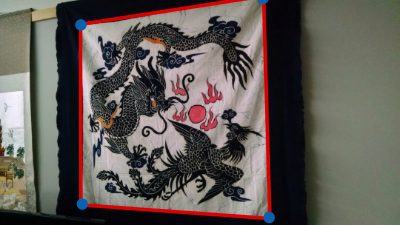
\includegraphics[width=.95\textwidth]{section01/assets/giftbox_1.png}
\subcaption[Captured Image]{\label{example1}}
\end{minipage}%
\begin{minipage}[t]{0.5\textwidth}
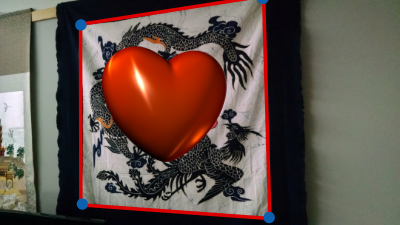
\includegraphics[width=.95\textwidth]{section01/assets/giftbox_2.png}
\subcaption[Mapping a Gift Onto the Image]{\label{example2}}
\end{minipage}%
\caption[Sample Result 2]{Conceptual Explanation of the AR System}
\end{figure}

\paragraph{} This application also contains a web interface that allows a user to view a description of the whole project before they download the Android application. In addition, users can view and edit their profile and also manage their friends list online. The web interface also allows you to check whether or not you have received new gifts.